\section{Анализ предметной области}
\subsection{Описание предметной области}
В настоящее время, когда население планеты продолжает расти, сельское хозяйство сталкивается с очень важной задачей -- обеспечение продовольственной безопасности. Поэтому поддержание здоровья сельскохозяйственных растений напрямую влияет на объемы и стабильность урожая \cite{plant5}.

На сегодняшний день, проблема защиты растений от болезней и вредителей по прежнему актуальна. По данным ФАО, по состоянию на 2024 год, потери сельскохозяйственных культур от вредителей и болезней растений достигают 40\%. В России ситуация также остается непростой: до 25\% зерновых культур гибнет из-за ржавчины, мучнистой росы, фузариоза и других заболеваний. Потери урожая картофеля из-за фитофтороза, альтернариоза и вирусных инфекций составляют 20–30\%. Рис страдает от пирикуляриоза, подсолнечник — от гнилей, сахарная свёкла — от церкоспороза, а яблони и сливы — от парши и монилиоза \cite{plant1}. Болезни растений, вызываемые разнообразными патогенами и неблагоприятными условиями, представляют собой серьезную угрозу для сельского хозяйства. Поэтому важно разработать эффективные методы их диагностики.

Традиционные методы для выявления болезней включают в себя несколько подходов:

\begin{enumerate}
	\item Визуальный осмотр: этот метод опирается на опыт и знания квалифицированных специалистов, предполагает анализ видимых симптомов, которые видны на различных частях растения \cite{plant6}.
	\item Микроскопический анализ: данная методика позволяет найти патогены в тканях растения. Для него используются оптические микроскопы, что помогает более точно определить источник заболевания \cite{plant2}.
	\item Молекулярные методы: этот метод исследования позволяет выявить генетические и молекулярные изменения в организме. Это обеспечивает высокую точность и специфичность диагностики \cite{plant10}.
\end{enumerate}

Однако, традиционные методы диагностики имеют свои ограничения. Они трудоемки, требуют использования специализированного оборудования и привлечения высококвалифицированных специалистов. Кроме того, их недостатками является то, что они могут потребовать много времени. Поэтому использование методов искусственного интеллекта и глубокого обучения может повысить точность и эффективность диагностики заболеваний сельскохозяйственных культур. \cite{vkr1}

\subsection{Роль искусственного интеллекта в сельском хозяйстве}
Искусственный интеллект находит всё более широкое применение в аграрном секторе. Его внедрение способствует снижению зависимости от ручного труда, оптимизации производственных процессов и повышению устойчивости агропроизводства перед лицом климатических и биотических рисков.

Одним из направлений применения ИИ является мониторинг состояния посевов. С использованием спутниковых и беспилотных летательных аппаратов, которые оснащённы высокоточным оптическим и мультиспектральным оборудованием, осуществляется регулярная съёмка посевов. Затем полученные изображения анализируются с помощью алгоритмов машинного и глубокого обучения для выявления отклонений в цвете, текстуре и структуре растений. Такой подход позволяют оперативно локализовать проблемные участки и сократить использование химических препаратов за счёт точечного воздействия \cite{vkr2}.

Ещё одно важное направление -- моделирование урожайности с помощью предсказания. На основе данных о метеоусловиях, составе почв, предыдущем урожае и многих других факторах формируются модели, способные предсказывать какой объём урожая может быть при текущих условиях . Эти системы активно применяются в странах ЕС, США, Китае и Индии для планирования сельскохозяйственных работ и оценки экономических рисков \cite{vkr1}.

Третье направление -- это диагностика заболеваний растений с использованием мобильных и веб-приложений. Эти платформы используют обученные сверточные нейронные сети, способные по фото растения сделать предположение о наличие конкретных заболеваний. Обучение таких моделей осуществляется на десятках тысяч размеченных изображений растений, которые пострадали от болезней или вредителей. Точность идентификации может превышать 90\%, что делает технологию полезной для мелких фермеров, не имеющих доступа к агрономам \cite{vkr3}.

Кроме того, активно развиваются роботизированные системы на базе ИИ, способные выполнять операции по уходу за растениям. Так, компании Naïo Technologies из Франции, Ecorobotix из Швейцарии, Small Robot Company из Великобритании разрабатывают автономных агророботов, которые смогут облегчить работу фермерам, путём автоматизации сложных и требующих высокой точности задач \cite{plant4}.

\subsection{Сверточные нейронные сети}

Сверточные нейронные сети (CNN, англ. Convolutional Neural Networks) представляют собой тип глубоких нейронных сетей, которые специально разработаны для обработки данных с сеточной структурой, таких как двумерные изображения. CNN кардинально изменили подход к анализу изображений, благодаря способности автоматически извлекать релевантные признаки из данных. Это сделало возможным решение таких задач, как классификация, сегментация, обнаружение и распознавание объектов с высокой точностью и устойчивостью к шумам и искажениям. 

Их основной принцип работы заключается в применении свёрточных фильтров, которые последовательно выявляют локальные закономерности в изображениях, начиная с простых признаков, таких как границы, и заканчивая высокоуровневыми абстракциями, такими как формы, контуры, объекты \cite{d21}.

Одной из первых архитектур, продемонстрировавших эффективность CNN, стала LeNet-5, разработанная Яном Лекуном в 1998 году для распознавания рукописных цифр. Она включала в себя два сверточных и два пулинг слоя, а также полносвязные слои на выходе. Несмотря на свою простоту, LeNet-5 продемонстрировала фундаментальные принципы, которые были заложены в более поздние архитектуры. На рисунке ~\ref{templ:image11} представлена архитектура LeNet-5. 
\begin{figure}[h]
	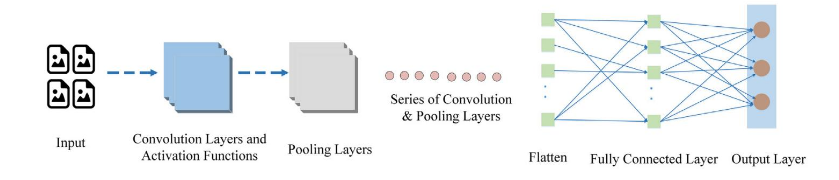
\includegraphics[width=1\linewidth]{lenet5.png}
	\caption{Архитектура LeNet-5}
	\label{templ:image11}
\end{figure}

Существенный прорыв в развитии сверточных сетей произошел, когда была разработана AlexNet в 2012 году. Она выиграла соревнование ImageNet, сократив ошибку классификации почти вдвое по сравнению с предыдущими моделями. AlexNet глубже использовала сверточные архитектуры, функцию активации ReLU, нормализацию по пакету и технику «дропаут» для уменьшения переобучения. Эта модель показала эффективность свёрточных сетей и стала катализатором их развития в целом. На рисунке ~\ref{templ:image12} представлена архитектура AlexNet.
\begin{figure}[h]
	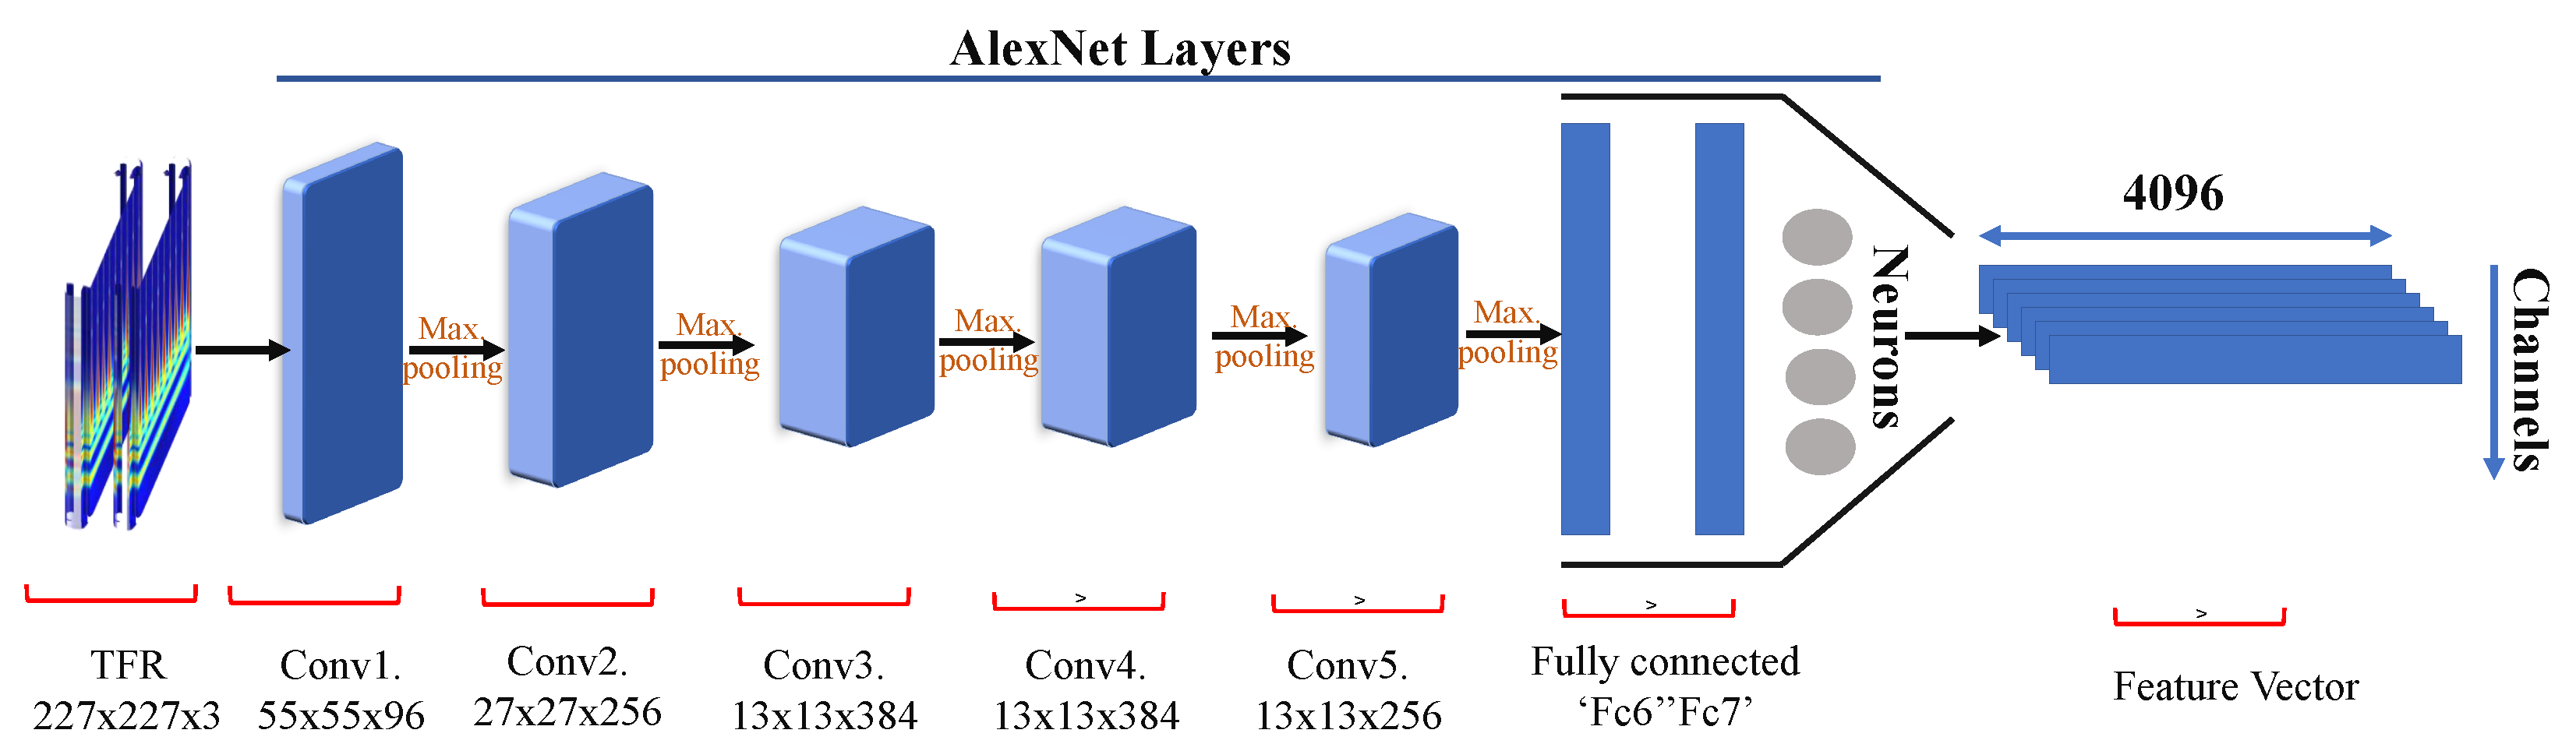
\includegraphics[width=1\linewidth]{alexnet.png}
	\caption{Архитектура AlexNet}
	\label{templ:image12}
\end{figure}

Впоследствии были разработаны более глубокие и эффективные архитектуры, такие как VGG, в которой использовались только 3×3 свёрток и 2×2 пуллинга, ResNet, в которой введены остаточные связи для облегчения обучения очень глубоких сетей, и GoogLeNet, которая использовала модули Inception. Эти модели стали стандартом в компьютерном зрении. Они применяются в различных отраслях: от медицины и промышленной диагностики до систем анализа спутниковых снимков. 

Развитие CNN позволило перейти от задач классификации к задачам более высокого уровня сложности, в частности к сегментации. Суть этой задачи заключается в построении пиксельных масок, которые соответствуют различным объектам или классам на изображении. Такой подход позволил расширить функциональность моделей по сравнению с обычной классификацией. Примерами соответствующих архитектур являются U-Net, DeepLab и Mask R-CNN, каждая из которых использует комбинацию сверточных и деконволюционных операций, а также механизмы пропуска слоев и многоуровневого объединения признаков \cite{d22}  .

Одним из ключевых направлений в развитии методов компьютерного зрения стало обнаружение объектов. Данная задача предполагает совместное решение задач классификации и локализации. Модель при этом должна не только определить принадлежность объекта к определённому классу, но и задать его пространственные координаты на изображении.

Для её  решения были разработаны архитектуры, сочетающие высокую производительность и точность. Наиболее известными моделями являются YOLO (You Only Look Once), SSD (Single Shot Multibox Detector) и Faster R-CNN. 

Первая из них представляет собой одноэтапную архитектуру. Она осуществляет предсказание координат и классов объектов в рамках единой свёрточной сети. Благодаря своей архитектуре, отличается высокой вычислительной эффективностью и возможностью обработки изображений в режиме, близком к реальному времени. 

Модель SSD тоже основана на одноэтапном подходе. Она использует многомасштабные карты признаков для распознавания объектов различных размеров, что делает её более универсальной при работе с разнородными данными. 

Faster R-CNN имеет двухэтапную архитектуру. Первый модуль генерирует предложений о потенциальной области объектов, а второй выполняет классификацию. Такой подход обеспечивает высокую точность за счёт явного разделения этапов локализации и распознавания.

\subsection{Анализ основных видов заболеваний томатов}

Томаты (Solanum lycopersicum) -- это одна из ключевых овощных культур, которую выращивают во всём мире. Она широко используется при приготовлении пищи и обладает высокой агрономической значимостью. В 2023 году мировое производство томатов составило более 190 млн тонн \cite{plant12}. Это показывает устойчивую тенденцию роста, даже на фоне климатических и биотических стрессов.

Однако томаты подвержены значительным потерям урожая из-за болезней и вредителей. Потери могут достигать 50\% в условиях высокой заболеваемости, особенно при отсутствии своевременного выявления заболеваний \cite{plant14} .

Одной из таких болезней является альтернариоз, или сухая пятнистость листьев. Это грибковое заболевание, вызываемое патогенами рода Alternaria, преимущественно Alternaria solani и Alternaria tomatophila. Заболевание поражает листья, стебли, плоды и приводит к значительным потерям урожая. 

Первые признаки болезни проявляются на нижних листьях в виде небольших тёмно-коричневых пятен с концентрическими кольцами. Со временем пятна увеличиваются, сливаются и охватывают большую часть листовой поверхности, вызывая преждевременное отмирание листьев. На стеблях и черешках появляются продольные тёмные полосы, которые могут приводить к их растрескиванию. На плодах появляются пятна гнили болотного цвета. 

Развитию болезни способствуют: высокая влажность воздуха, температура в диапозоне от +20$^{\circ}$C до +30$^{\circ}$C, густая посадка, мешающая циркуляции воздуха. Споры гриба могут сохраняться в почве и на растительных остатках до 2–3 лет, поэтому необходимо соблюдать севооборот и тщательно убирать поля после сбора урожая \cite{plant2}. На рисунке ~\ref{templ:image1} представлены признаки болезни на листьях.
\begin{figure}[h]
	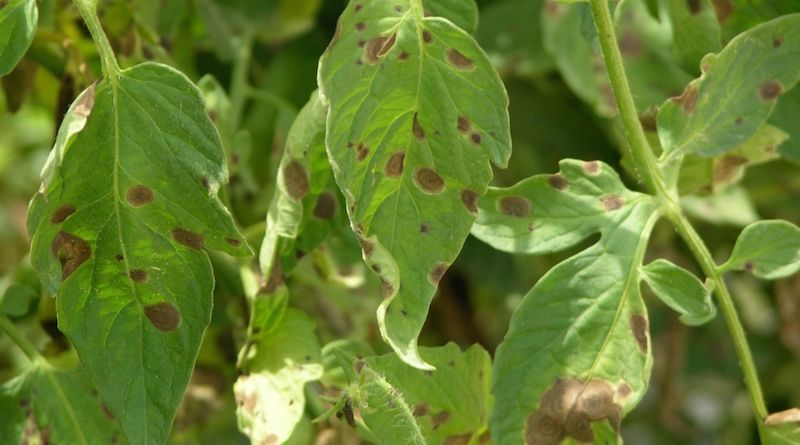
\includegraphics[width=1\linewidth]{альтерниоз tomatov.jpg}
	\caption{Альтернариоз}
	\label{templ:image1}
\end{figure}

Одним из наиболее опасных заболеваний томатов является фитофтороз, вызываемый оомицетом Phytophthora infestans. Эта патогенная микроскопическая структура также поражает картофель и другие растения семейства паслёновых. Фитофтороз способен стремительно распространяться в условиях высокой влажности и умеренных температур, вызывая массовое заражение посадок и значительное снижение урожайности.

Первые признаки заболевания появляются на нижних листьях в виде водянистых пятен бурого или серо-зелёного цвета. По мере развития болезни пятна становятся более выраженными, часть листа вокруг них отмирает, и образуется светлый ободок. С нижней стороны листьев может наблюдаться белый налёт, представляющий собой мицелий патогена. Поражение распространяется вверх по растению. Оно охватывает стебли и плоды. На плодах фитофтороз вызывает бурые, твёрдые пятна, часто с чёрной каймой. Такие плоды быстро загнивают, особенно в условиях хранения \cite{plant3}.
На рисунке ~\ref{templ:image2} представлены признаки болезни на листьях.
\begin{figure}[h]
	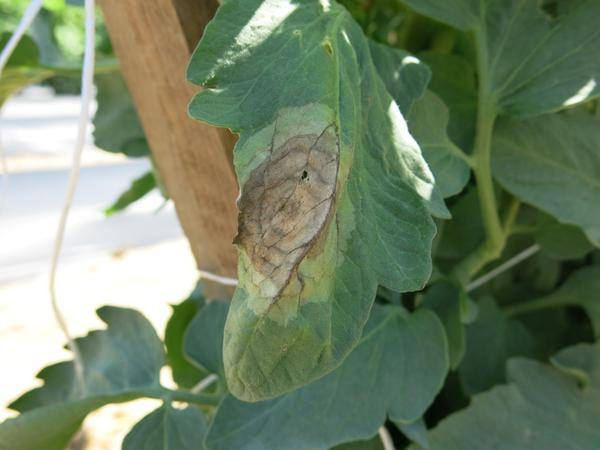
\includegraphics[width=1\linewidth]{late-blight-foliage-tomato.jpg}
	\caption{Фитофтороз}
	\label{templ:image2}
\end{figure}

Кладоспориоз томатов, также известный как бурая пятнистость, — это грибное заболевание. Патоген поражает преимущественно листья томатов, реже -- стебли и плодоножки. У болеющего томата значительно снижается урожайность и качество самих плодов.

Болезнь вызывается грибом Cladosporium fulvum, который развивается на межклеточном уровне и продуцирует токсины, нарушающие физиологические процессы в растении. Грибки распространяется спорами, которые разносятся с потоками воздуха, а также через инструменты, одежду или капли воды. Также источником инфекции могут быть заражённые растительные остатки или семена, не прошедшие предварительную обработку \cite{plant11}.

Наиболее характерные признаки кладоспориоза проявляются на нижней стороне листьев в виде светло-зелёных, жёлтых, а затем бурых пятен округлой или неправильной формы. На рисунке ~\ref{templ:image3} представлено больное растение. Поражённые листья постепенно скручиваются, усыхают и опадают.

\begin{figure}[h]
	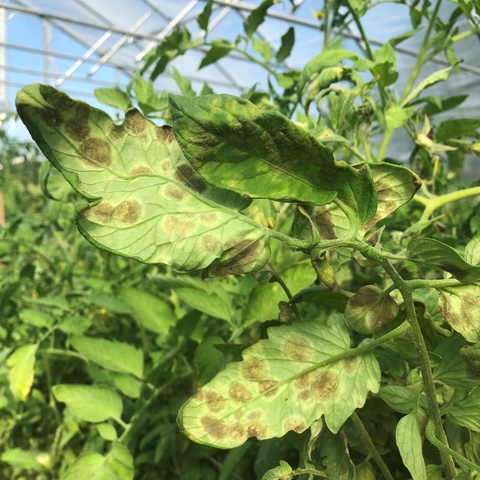
\includegraphics[width=1\linewidth]{кладоспориоз-томата-2-e1598945034942.jpg}
	\caption{Кладоспориоз}
	\label{templ:image3}
\end{figure}

Септориоз томатов, или белая пятнистость, -- это одно из наиболее распространённых грибных заболеваний, вызываемое патогеном Septoria lycopersici Speg. Болезнь поражает преимущественно листву в фазу активного роста растений.

По данным специалистов Россельхозцентра, септориоз регистрируется ежегодно во всех регионах России, но чаще всего в зонах с повышенной влажностью \cite{plant8}.

Первые признаки проявляются на нижних листьях в виде маленьких светло-серых пятен с тёмной каймой. Постепенно пятна увеличиваются до 2–5 мм в диаметре, становятся округлыми, с отчетливо выраженной тёмной границей. В центре пятен можно разглядеть мелкие тёмные точки — пикниды гриба. Изображение больного листа представлено на рисунке ~\ref{templ:image4}.

\begin{figure}[h]
	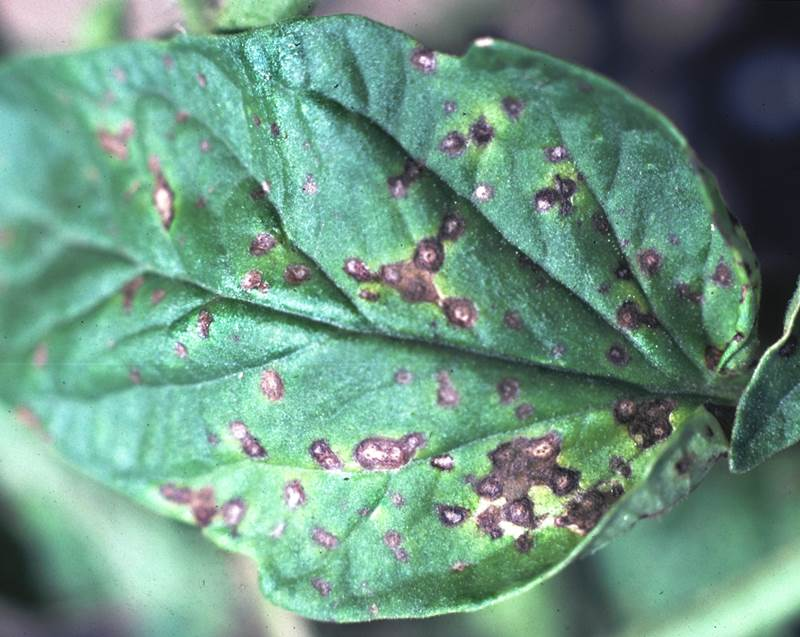
\includegraphics[width=1\linewidth]{4.jpg}
	\caption{Септориоз томата}
	\label{templ:image4}
\end{figure}

При сильном развитии болезни пятна сливаются, листовая пластинка желтеет, высыхает и опадает. Это нарушает фотосинтез и ослабляет растение, особенно в период формирования завязей.

Мозаичный вирус томатов -- одно из наиболее известных и широко распространённых вирусных заболеваний томатов. Болезнь отличается высокой заразностью и может вызвать значительное снижение урожайности и ухудшение качества плодов.

Вирус впервые был описан в начале XX века. Возбудитель относится к роду Tobamovirus и представляет собой устойчивую РНК-вирусную частицу \cite{plant19}.

Первые признаки заражения чаще всего появляются на молодых листьях. Они приобретают характерную мозаичную окраску, при которой чередуются светло-зелёные и тёмно-зелёные участки. На стеблях и черешках появляются бурые полосы, а плоды теряют равномерность окраски и могут быть покрыты кольцевыми пятнами. В условиях высокой температуры и интенсивного солнечного света симптомы становятся более выраженными. Изображение зараженного томата представлено на рисунке ~\ref{templ:image5}.
\begin{figure}[h]
	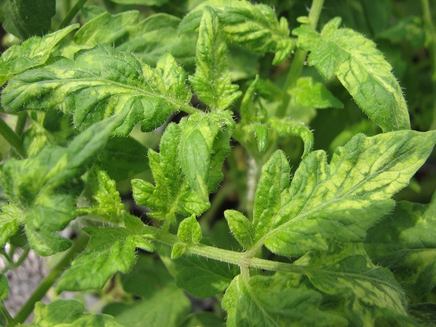
\includegraphics[width=1\linewidth]{pepino-mosaic-virus(4).jpg}
	\caption{Мозаичный вирус}
	\label{templ:image5}
\end{figure}

Передача вируса происходит через контакт с руками, одеждой, садовым инвентарём, на которых есть вирус, или при контакте с насекомыми-переносчиками, такими как тля и табачный трипс \cite{plant5}.

Вирус жёлтой курчавости листьев томата -- ещё одно опасное вирусных заболеваний. Он относится к роду Begomovirus, семейству Geminiviridae, и характеризуется способностью к быстрому распространению, особенно в регионах с тёплым климатом.

На территории России заболевание наиболее часто встречается в южных регионах — Краснодарском крае, Ростовской области, Крыму и Ставрополье, где благоприятные климатические условия способствуют активному размножению основного переносчика -- белокрылки (Bemisia tabaci). Она является единственным распространителем данного вируса \cite{plant13}. Изображение зараженного томата представлено на рисунке ~\ref{templ:image6}.
\begin{figure}[h]
	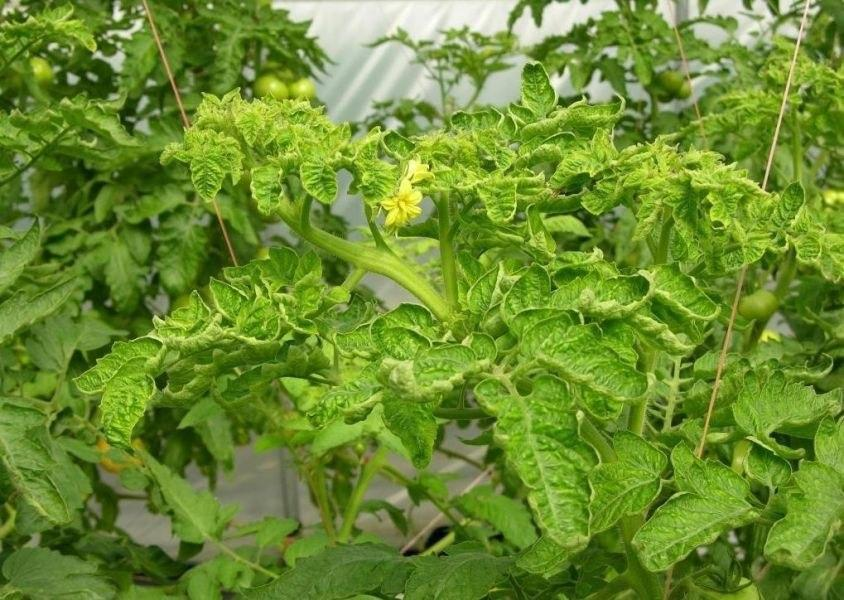
\includegraphics[width=1\linewidth]{Tomato-Yellow-Leaf-4.jpg}
	\caption{Вирус жёлтой курчавости}
	\label{templ:image6}
\end{figure}

У заражённых растений листья уменьшаются в размере, становятся ломкими, закручиваются вверх и приобретают лимонно-жёлтую окраску. Снижается способность к фотосинтезу, и, как следствие, ограничивается формирование цветков и завязей, что приводит к недостаточному развитию плодов или полному отсутствию урожая\cite{plant14}.

Минирующая мушка -- один из опаснейших вредителей овощных культур. Они наносят серьёзный вред растениям, как на стадии рассады, так и в период плодоношения. Эти мелкие двукрылые насекомые относятся к семейству Agromyzidae и отличаются высокой плодовитостью и быстрой адаптацией к инсектицидам. На изображении ~\ref{templ:image7} представлена минирующая мушка \cite{plant15}. 

\begin{figure}[h]
	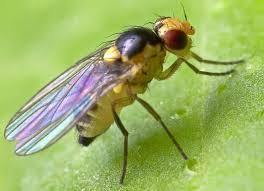
\includegraphics[width=1\linewidth]{муха.jpeg}
	\caption{Минирующая мушка}
	\label{templ:image7}
\end{figure}


Самки прокалывают эпидермис листьев для откладки яиц. Вылупившиеся личинки начинают проделывать ходы в мезофилле листа, и, тем самым, разрушают фотосинтетическую ткань. Визуально повреждения проявляются в виде извилистых светлых линий -- мин, которые увеличиваются в размерах по мере роста личинки. Повреждения представлены на изображении ~\ref{templ:image8}. При высокой численности вредителя может быть снижение урожайности до 40\% [ссылка]ФГБУ «Россельхозцентр», 2021).

\begin{figure}[h]
	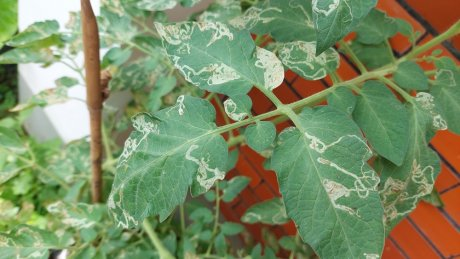
\includegraphics[width=1\linewidth]{мин мушка.jpg}
	\caption{"Мины"}
	\label{templ:image8}
\end{figure}

Мушки особенно опасны в теплицах, где температурно-влажностные условия способствуют быстрому размножению. В одном поколении может развиваться до 600–700 яиц, а полный цикл развития при благоприятных условиях занимает 15–20 дней.

Паутинный клещ -- один из наиболее опасных вредителей, поражающих более 200 видов растений, включая томаты. Его биология, малые размеры и высокая устойчивость к пестицидам делают борьбу с ним крайне сложной [ссылка]. Особь клеща представлена на изображении ~\ref{templ:image9}.

Развитие клеща проходит особенно интенсивно при температуре 25–30 $^{\circ}$C и относительной влажности менее 60\%. Полный цикл развития — от яйца до взрослой особи — может занимать всего 7–10 суток, что позволяет вредителю развивать до 20 поколений в год в теплицах. Самки откладывают до 100–150 яиц за жизнь, формируя плотные колонии в межжилковых пространствах листьев \cite{plant18}.

\begin{figure}[h]
	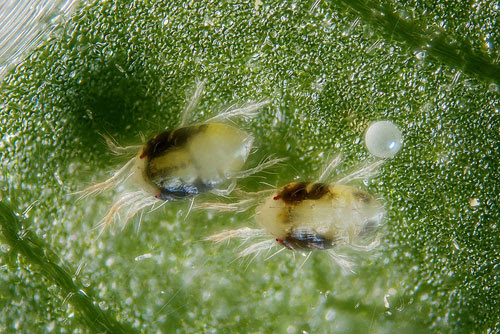
\includegraphics[width=1\linewidth]{клещ.jpg}
	\caption{Паутинный клещ}
	\label{templ:image9}
\end{figure}

На томатах паутинный клещ вредит в основном с нижней стороны листьев, прокалывая эпидермис и высасывая клеточный сок. Первичные симптомы проявляются в виде мелких светлых точек -- хлорозов, которые со временем сливаются и придают листьям мраморный вид. При сильной степени заражения листья буреют, скручиваются, засыхают и опадают. Также можно наблюдать тонкую паутину, покрывающую нижнюю сторону листьев, черешки и даже соцветия. Паутина служит защитой для колоний клещей и яиц от внешних воздействий и инсектицидов [ссылка](Минаев, 2018). На изображении ~\ref{templ:image10} представлен, томатный куст, пострадавший от клещей.

\begin{figure}[H]
	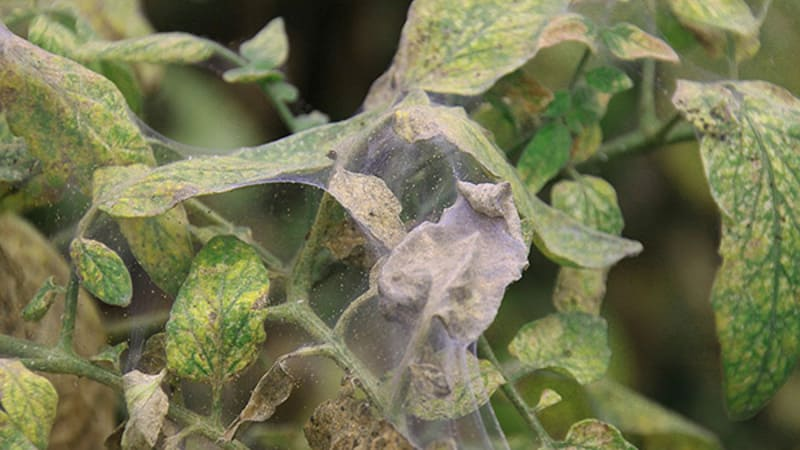
\includegraphics[width=1\linewidth]{паут кл2.jpeg}
	\caption{Колония паутинных клещей на кусте томата}
	\label{templ:image10}
\end{figure}

\subsection{Анализ существующих решений}
С помощью анализу существующих решений с похожей тематикой, можно выделить их достоинства и недостатки, чтобы использовать эту информацию при разработке своего решения. 
Были выбраны три веб-сервиса, в которых используются технологии компьютерного зрения и искусственного интеллекта:
\begin{itemize}
	\item "plantix";
	\item  "cultiKure";
	\item "pdd.jinr".
\end{itemize}
Все указанные платформы решают задачи идентификации болезней растений по загруженным изображениям, однако имеют отличия в интерфейсе, используем технологиях и функционале.

Так Plantix -- это мобильное приложение, ориентированное на фермеров и агрономов. пользователь делает фото растения, а приложение анализирует его и предоставляет подробную информацию о заболевании, методах лечения. Интерфейс рассчитан на массового пользователя и поддерживает множество региональных языков. Однако его минусом является то, что это мобильное приложение, поэтому нет возможности использовать его через браузер. На изображении ~\ref{templ:image13} представлен страница Plantix.

\begin{figure}[ht]
	\centering
	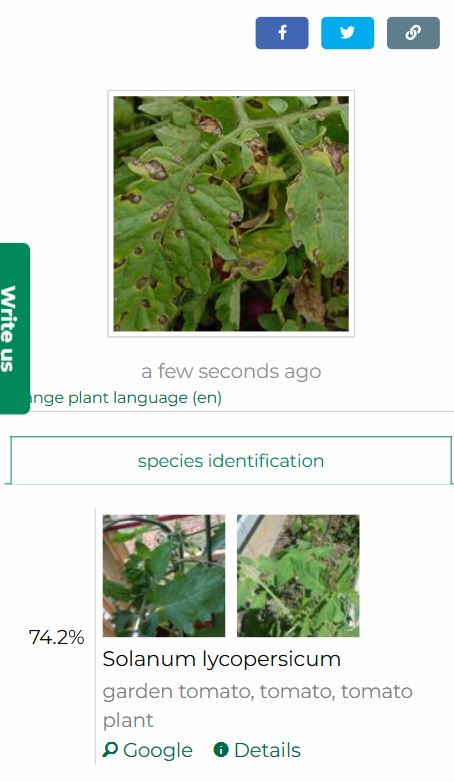
\includegraphics[width=0.5\linewidth]{платекс.png}
	\caption{Интерфейс Plantix}
	\label{templ:image13}
\end{figure}

CultiKure -- это веб-приложение, предназначенное для помощи пользователям в выявлении и устранении заболеваний растений. Оно анализирует изображения листьев с помощью модели VGG16 и выдаёт результаты с информацией по болезням. Само приложение построено на базе фреймворка Flask. Минусом данного решения является то, что оно использует не самую лучшую версию модели, и, как результат, может выдавать не самые точные предсказания \cite{cn1}.
На изображении ~\ref{templ:image14} представлен страница CultiKure.

\begin{figure}[H]
	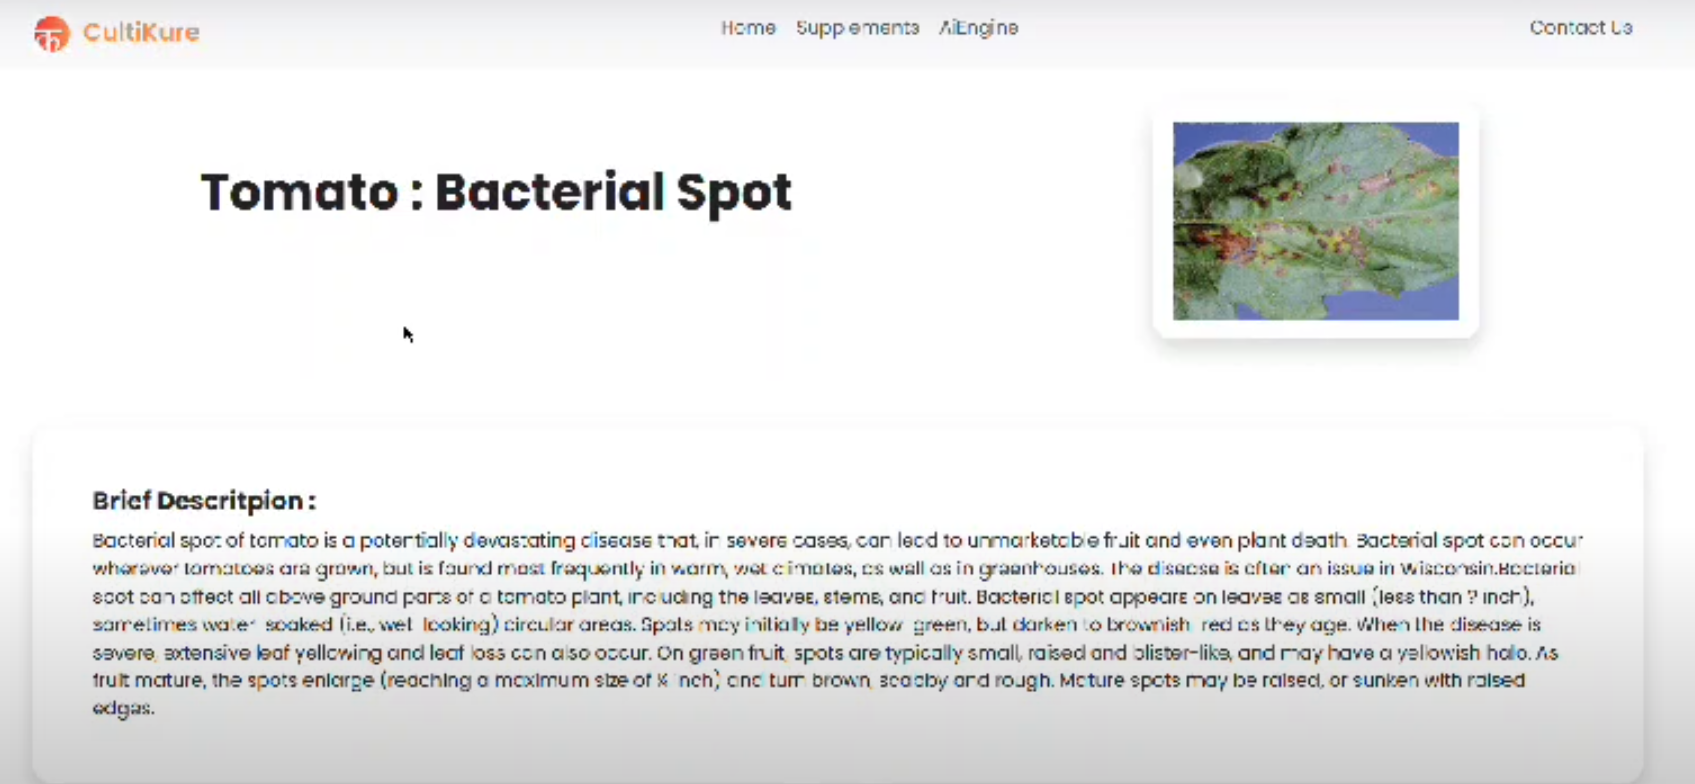
\includegraphics[width=1\linewidth]{култикури.png}
	\caption{Интерфейс CultiKure}
	\label{templ:image14}
\end{figure}

PDD.JINR.RU является исследовательским проектом, созданным в "Объединённом институте ядерных исследований". Веб-интерфейс позволяет загружать изображения листьев и определять заболевание с помощью сверточной нейросети. Акцент данного решения делается на точность и демонстрацию работы алгоритма ИИ. Однако визуальное оформление сайта значительно уступает в удобстве и современности свои конкурентам. На изображении ~\ref{templ:image15} представлен интерфейс, а на ~\ref{templ:image16} - результат предсказания PDD.JINR.RU.

\begin{figure}[H]
	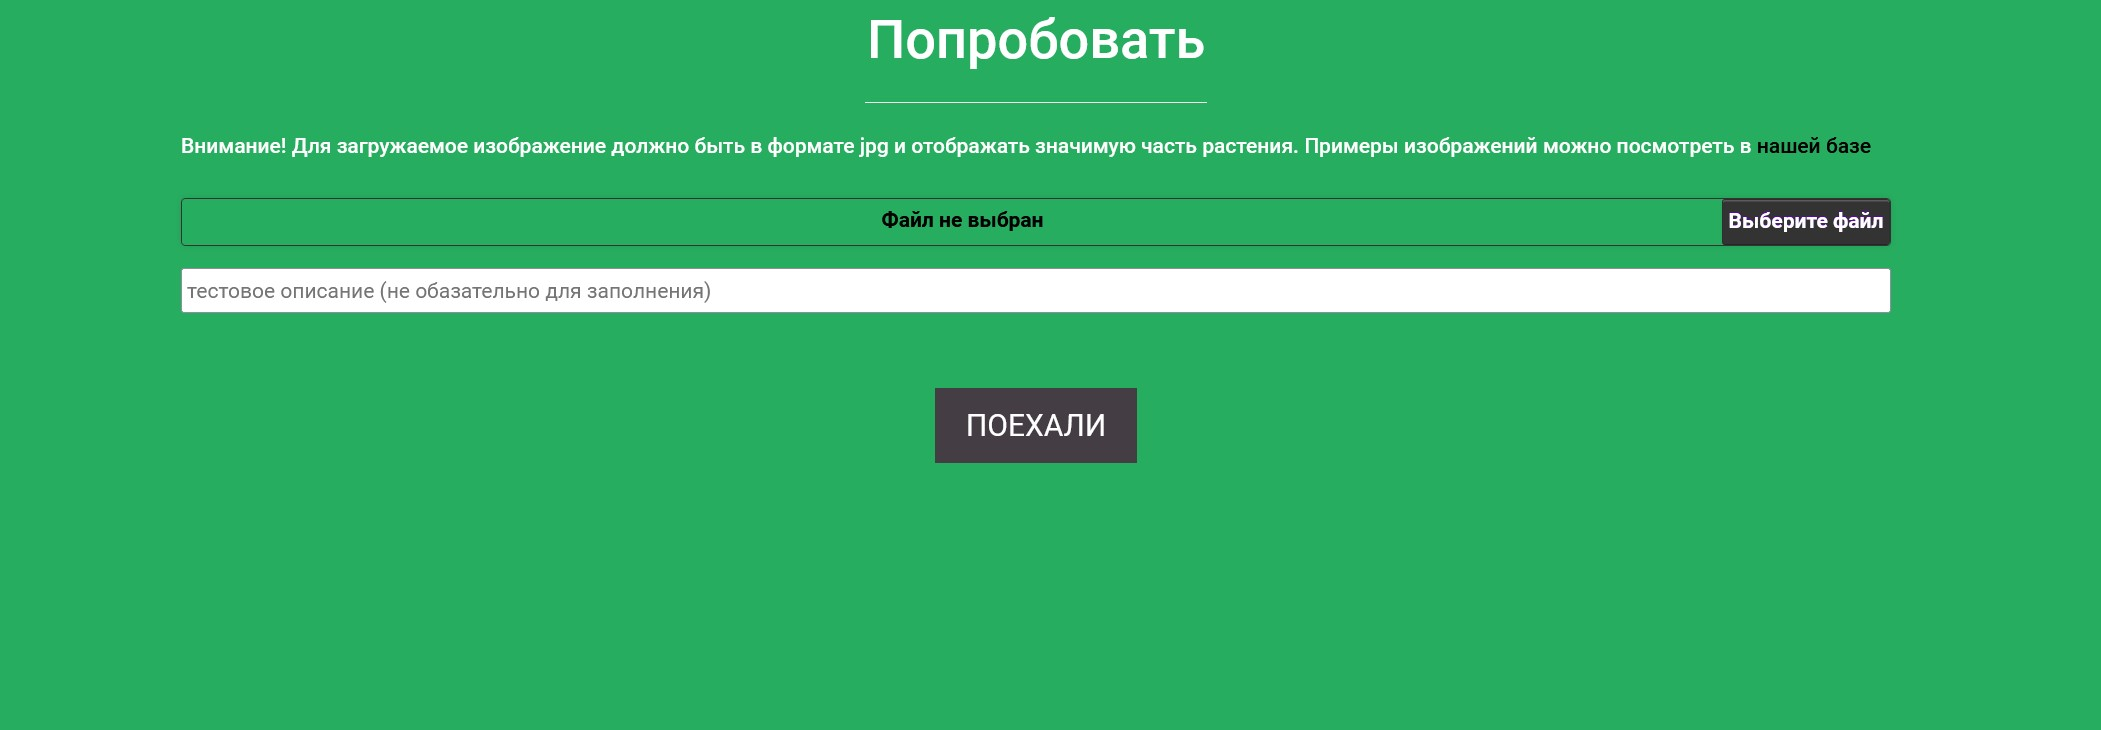
\includegraphics[width=1\linewidth]{site1.jpg}
	\caption{Интерфейс PDD.JINR.RU}
	\label{templ:image15}
\end{figure}


\begin{figure}[H]
	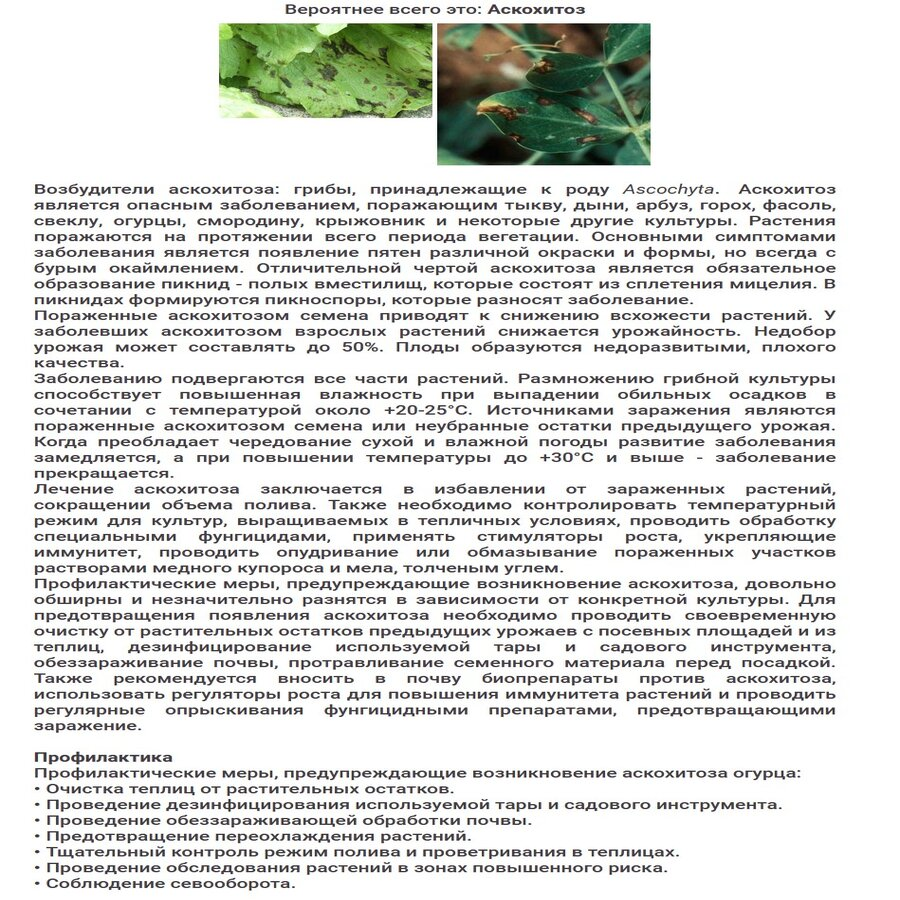
\includegraphics[width=0.9\linewidth]{site2.jpg}
	\caption{Интерфейс PDD.JINR.RU}
	\label{templ:image16}
\end{figure}


